
\documentclass[12pt,a4paper]{book}
\usepackage[minitoc]{teach}
\usepackage[utf8]{inputenc}
\usepackage[french]{babel}
\usepackage[T1]{fontenc}
\usepackage{amsmath}
\usepackage{amsfonts}
\usepackage{amssymb}
\usepackage{graphicx}
\pagestyle{fancy}
\renewcommand{\headrulewidth}{0pt}
\renewcommand{\footrulewidth}{0pt}


\author{YAWO Kossi Atsu}
\newcommand{\prof}{YAWO Kossi Atsu}
\newcommand{\matiere}{MATHEMATIQUES}
\newcommand{\classe}{6$^{ème}$}
\title{Mes devoirs de Mathématiques}
\begin{document}

\begin{devoir}{DEVOIR SURVEILLE DU PREMIER TRIMESTRE}{\matiere}{\classe}{1}{1H 30}{13 novembre 2019}{\prof}
\begin{exo}[8]
En 2017, l'Organisation des Nations Unies (ONU) a donné la répartition suivante de la population mondiale:
% \usepackage{array} is required
\begin{tabular}{|l|>{\raggedright\arraybackslash}p{13cm}|}
\hline 
\textbf{Zone géographique}  & \textbf{Population} \\ 
\hline 
Europe & 742074000 \\ 
\hline 
Océanie & quarante millions six cent quatre-vingt-onze mille \\ 
\hline 
Amérique latine et Caraïbes & 645593000 \\ 
\hline 
Asie & quatre milliards cinq cent quatre millions quatre cent vingt-huit mille \\ 
\hline 
Antarctique & 1500 \\ 
\hline 
Afrique & 1256268000 \\ 
\hline 
Etats-Unies et Canada & 361208000 \\ 
\hline 
\end{tabular} 

\vspace{0.5cm}
\textbf{\underline{Consignes}:}
\begin{enumerate}
\item Quelle est la zone du monde la plus plus peuplée?
\item Quelle est la zone du monde la moins peuplée?
\item Yaovi, un élève de la classe de 6ème pense que l'Europe est plus peuplé que l'Afrique. A-t-il raison?
\end{enumerate}

\vspace{0.5cm}

\begin{tabular}{|c|c|c|c|c|}
\hline 
Critère & Pertinence & Correction & Cohérence & Perfectionnement \\ 
\hline
Barème & 2pts & 2pts & 3pts & 1pt \\ 
\hline 
\end{tabular}
\competence{•}{8}
\end{exo}
 
\vspace{0.5cm}
\begin{exo}[4]
\begin{defitemize}
\item Choisi la bonne réponse:
\begin{multicols}{2}
\begin{enumerate}
\item Le nombre entier naturel qui précède 999 est:
\begin{enumerate}
\item 998
\item 1000
\item 99,8
\end{enumerate}
\item L'écriture décimale de $\frac{123}{100}$ est:
\begin{enumerate}
\item 0,123
\item 1,23
\item 12,3
\end{enumerate}
\item La partie décimal e 45,12 est:
\begin{enumerate}
\item 0,12
\item 12
\item 45
\end{enumerate}
\item La partie entière de 25,002:
\begin{enumerate}
\item 0,002
\item 25
\item 2
\end{enumerate}

\end{enumerate}
\end{multicols}

\item Réponds par vrai ou faux
\begin{enumerate}
\item $1235 \in \mathbb{N}$
\item $0,13 \notin \mathbb{N}$ 
\item $\frac{8}{2} \notin \mathbb{N}$
\item $0 \notin \mathbb{N}$
\end{enumerate}
\competence{•}{2}
\end{defitemize}
\end{exo}

\begin{exo}[8]
\begin{enumerate}
\item Trace deux droites $(D_1)$ et $(D_2)$ perpendiculaires en A. Marque un point $B$ appartenant à $(D_1)$ et un point $C$ appartenant à $(D_2)$. Trace la droite $(D_3)$ passant par $A$ et perpendiculaire à $(BC)$ en $D$.
\begin{enumerate}
\item Que peux tu dire des points $B$, $C$ et $D$?
\item Trace la droite $(D_4)$, perpendiculaire à $(D_1)$ en $B$. Que peux- tu dire des droites $(D_4)$ et $(D_2)$? Justifie.
\end{enumerate}
\competence{•}{4}
\item On te propose la figure ci-contre.
\begin{multicols}{2}
Marque:
\begin{defitemize}
\item un point $L$ tel que $O$, $I$ et $L$ soient alignés.
\item un point $M$ tel que $O$, $J$ et $M$ soient alignés.
\item un point $N$ tel que $I$, $K$ et $N$ soient alignés.
\item un point $P$ tel que $I$, $J$ et $P$ soient alignés.
\end{defitemize}

Recopie puis complète par un nom de droite qui convient:\\
$L \in (\ldots)$ \qquad ;\qquad $M \in (\ldots)$ \qquad ;\qquad $N \in (\ldots)$ \qquad ;\qquad $P \in (\ldots)$

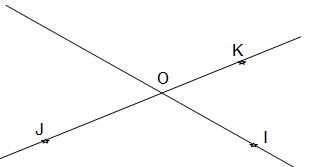
\includegraphics[scale=0.9]{images/dev120192020img1.png}
\end{multicols}

\competence{•}{4}
\end{enumerate}
\end{exo}

\tableofcompetences
\end{devoir}

\newpage

\begin{td}{\matiere}{\classe}{23 novembre 2019}{\prof}
\begin{exo}
\begin{enumerate}
\item Ecris en chiffres:
\begin{remslist}
\item Onze mille vingt neuf.
\item trois unités quatre-vingt-cinq centièmes.
\item Douze unités quatre millièmes. 
\end{remslist}
\item On considère le nombre $A=146952783$
\begin{enumerate}
\item Réécris ce nombre en regroupant les chiffres de façon à rendre plus facile sa lecture.
\item Ecris ce nombre en lettres.
\item Quel est le chiffre:
\begin{remslist}
\item des unités?
\item des dizaines?
\item des centaines de milliers?
\item des dizaines de millions?
\end{remslist}
\end{enumerate}
\item Quel est le nombre dont le chiffre des dizaines est 7, le chiffre des dixièmes est 6, le chiffre des centaines et le chiffre des centièmes est 3 et dont les autres sont nuls?
\item L'écriture $3 \times 5$ montre que ce nombre est un multiple de 3. En utilisant une écriture du même type que $3 \times 5$:
\begin{enumerate}
\item écris le multiple de 3 qui précède $3 \times 5$.
\item écris le multiple de 3 qui suit $3 \times 5$.
\end{enumerate}
\item Range les nombres décimaux suivants par l'ordre croissant:\\
$42$ \qquad ; \qquad $41,22$ \qquad ; \qquad $42,12$ \qquad ; \qquad $42,3$ \qquad ; \qquad $42,27$ \qquad ; \qquad $41,05$ \qquad ; \qquad $42,001$ \qquad et \qquad $41$
\end{enumerate}
\end{exo}

\vspace{1cm}

\begin{exo}
On donne la figure ci-dessous:\\

\includegraphics[scale=0.9]{images/td1img1.png}
\begin{enumerate}
\item Donne un autre nom à la demi-droite $[CF)$.
\item Donne deux autres noms de la demi-droite d'origine $C$ qui passe par le point $A$.
\item Quelle est la demi-droite opposée à la demi-droite $[AB)$.
\item Complète par $\in$ ou $\notin$:\\
$A \ldots [AB)$ \qquad ; \qquad $E \ldots [AB)$ \qquad ; \qquad $F \ldots [AB)$ \qquad et \qquad $C \ldots [AB)$
\end{enumerate}
\end{exo}

\vspace{1cm}
\begin{exo}
Trace deux droites sécantes $(OG)$ et $(OE)$.
\begin{enumerate}
\item On désire ensuite marquer le point M tel que $(EM) \perp (OE)$ et $(GM)//(OE)$. Explique comment peux-tu procéder.
\item Justifie à l'aide d'un déductogramme que les droites $(EM)$ et $(GM)$ sont perpendiculaires.
\end{enumerate} 
\end{exo}
\end{td}

\newpage
\begin{devoir}{COMPOSITION DU PREMIER TRIMESTRE}{\matiere}{\classe}{1}{1H 30}{13 décembre 2019}{\prof}
\begin{exo}[5]
\begin{multicols}{2}
On considère le nombre ci-contre. Il est composé de cinq chiffres dont deux sont masqués. On sait aussi qu'il est divisible par 2, par 3 et par 5.
Quel peut être ce nombre? Donne toutes les possibilités en justifiant tes réponse.
\begin{center}

\includegraphics[scale=0.9]{images/compo1img1.png}
\end{center}
\vspace{1cm}
.
\end{multicols}
\competence{•}{5}
\end{exo}

\begin{exo}[8]
\begin{multicols}{2}
\begin{enumerate}
\item Ecris en chiffres:
\begin{remslist}
\item Onze mille vingt neuf.
\item trois unités quatre-vingt-cinq centièmes.
\item Douze unités quatre millièmes. 
\end{remslist}
\item On considère le nombre $A=146952783$
\begin{enumerate}
\item Réécris ce nombre en regroupant les chiffres de façon à rendre plus facile sa lecture.
\item Ecris ce nombre en lettres.
\item Quel est le chiffre:
\begin{remslist}
\item des unités?
\item des dizaines?
\item des centaines de milliers?
\item des dizaines de millions?
\end{remslist}
\end{enumerate}
\item Quel est le nombre dont le chiffre des dizaines est 7, le chiffre des dixièmes est 6, le chiffre des centaines et le chiffre des centièmes est 3 et dont les autres sont nuls?
\item L'écriture $3 \times 5$ montre que ce nombre est un multiple de 3. En utilisant une écriture du même type que $3 \times 5$:
\begin{enumerate}
\item écris le multiple de 3 qui précède $3 \times 5$.
\item écris le multiple de 3 qui suit $3 \times 5$.
\end{enumerate}
\item Range les nombres décimaux suivants par l'ordre croissant:\\
$42$ \qquad ; \qquad $41,22$ \qquad ; \qquad $42,12$ \qquad ; \qquad $42,3$ \qquad ; \qquad $42,27$ \qquad ; \qquad $41,05$ \qquad ; \qquad $42,001$ \qquad et \qquad $41$
\end{enumerate}
\end{multicols}
\competence{•}{8}
\end{exo}

\vspace{0.5cm}

\begin{exo}[4]
On donne la figure ci-dessous:\\

\includegraphics[scale=0.9]{images/td1img1.png}
\begin{enumerate}
\item Donne un autre nom à la demi-droite $[CF)$.
\item Donne deux autres noms de la demi-droite d'origine $C$ qui passe par le point $A$.
\item Quelle est la demi-droite opposée à la demi-droite $[AB)$.
\item Complète par $\in$ ou $\notin$:\\
$A \ldots [AB)$ \qquad ; \qquad $E \ldots [AB)$ \qquad ; \qquad $F \ldots [AB)$ \qquad et \qquad $C \ldots [AB)$
\end{enumerate}
\competence{•}{4}
\end{exo}

\vspace{0.5cm}
\begin{exo}[3]
Trace deux droites sécantes $(OG)$ et $(OE)$.
\begin{enumerate}
\item On désire ensuite marquer le point M tel que $(EM) \perp (OE)$ et $(GM)//(OE)$. Explique comment peux-tu procéder.
\item Justifie à l'aide d'un déductogramme que les droites $(EM)$ et $(GM)$ sont perpendiculaires.
\end{enumerate} 
\competence{•}{3}
\end{exo}

\tableofcompetences
\end{devoir}

\newpage
\begin{td}{\matiere}{\classe}{$1^{er}$ février 2020}{\prof}
\begin{exo}
\begin{enumerate}
\item Trace un segment $[AB]$ de longueur $6cm$. Nomme C son milieu.
\item Trace la droite $(D_1)$ perpendiculaire à $(AB)$ et passant par C. Que peux-tu dire de cette droite? Justifie.
\item Place un point D de $(D_1)$ distinct de $C$.
\begin{enumerate}
\item Compare les distances $AD$ et $CD$. Justifie ta réponse.
\item Quelle est la nature du triangle ABC?
\end{enumerate}
\item Trace la droite $(D_2)$ passant par B et perpendiculaire à $(AB)$.Elle coupe la droite $(AC)$ en E.
\begin{enumerate}
\item Que peux tu dire des droites $(D_1)$ et $(D_2)$? Justifie.
\item Que peux-tu dire des points A, C et E?
\end{enumerate} 
\item Trace la droite $(D3)$ passant par A et parallèle à $(D_1)$.
\item Justifie que les droite $(D_3)$ et $(D_2)$.
\end{enumerate} 
\end{exo}
\end{td}

\vspace{3cm}

\begin{td}{\matiere}{\classe}{$1^{er}$ février 2020}{\prof}
\begin{exo}
\begin{enumerate}
\item Trace un segment $[AB]$ de longueur $6cm$. Nomme C son milieu.
\item Trace la droite $(D_1)$ perpendiculaire à $(AB)$ et passant par C. Que peux-tu dire de cette droite? Justifie.
\item Place un point D de $(D_1)$ distinct de $C$.
\begin{enumerate}
\item Compare les distances $AD$ et $CD$. Justifie ta réponse.
\item Quelle est la nature du triangle ABC?
\end{enumerate}
\item Trace la droite $(D_2)$ passant par B et perpendiculaire à $(AB)$.Elle coupe la droite $(AC)$ en E.
\begin{enumerate}
\item Que peux tu dire des droites $(D_1)$ et $(D_2)$? Justifie.
\item Que peux-tu dire des points A, C et E?
\end{enumerate} 
\item Trace la droite $(D3)$ passant par A et parallèle à $(D_1)$.
\item Justifie que les droite $(D_3)$ et $(D_2)$ sont parallèles.
\end{enumerate} 
\end{exo}
\end{td}

\newpage
\begin{devoir}{DEVOIR SURVEILLÉ DU DEUXIÈME TRIMESTRE}{\matiere}{\classe}{2}{1H 30'}{12 février 2020}{\prof}
\begin{exo}[8pts]
L'organisateur d'une fête scolaire commande 48 casiers de boisson gazeuse et 100 boîtes de jus d'ananas. Il y a 24 bouteilles dans chaque casier. En déchargeant le camion, le convoyeur casse 6 bouteilles. Ces bouteilles ne seront pas payées par l'organisateur. \\ Sachant qu'une bouteille de boisson gazeuse coûte 200 francs et une boîte de jus d'ananas 300 francs, combien l'organisateur devra-t-il payer au fournisseur?
\end{exo}

\vspace{1cm}

\begin{exo}[6]
\begin{enumerate}
\item 783 est un multiple de 29.
\begin{enumerate}
\item Écris le multiple de 29 qui précède 783.
\item Écris le multiple de 29 qui suit 783.
\end{enumerate}
\item \begin{enumerate}
\item Ecris une phrase qui a la même signification que: "91 est un multiple de 7".
\item Traduis cette phrase par une égalité.
\item l'égalité précédente montre 91 est aussi divisible par un autre nombre entier naturel, lequel?
\end{enumerate}
\item Reproduis puis complète le tableau suivant:\\
\begin{tabular}{|c|c|c|c|c|c|}
\hline 
75 & 100 & 123 & 783 & 6300 & est divisible par \\ 
\hline 
 &  &  &  &  & 1 \\ 
\hline 
 & &  &  &  & 2 \\ 
\hline 
 &  & &  &  & 3 \\ 
\hline 
 &  &  &  &  & 5 \\ 
\hline 
 &  &  &  &  & 9 \\ 
\hline 
 & & &  &  & 10 \\ 
\hline 
 &  &  &  &  & 100 \\ 
\hline 
\end{tabular} 
\end{enumerate}
\end{exo}

\vspace{1cm}

\begin{exo}[6]
\begin{enumerate}
\item Trace un segment $[AB]$ de longueur $6cm$. Nomme C son milieu.
\item Trace la droite $(D_1)$ perpendiculaire à $(AB)$ et passant par C. Que peux-tu dire de cette droite? Justifie.
\item Place un point D de $(D_1)$ distinct de $C$.
\begin{enumerate}
\item Compare les distances $AD$ et $BD$. Justifie ta réponse.
\item Quelle est la nature du triangle DBA?
\end{enumerate}
\item Trace la droite $(D_2)$ passant par B et perpendiculaire à $(AB)$.Elle coupe la droite $(AD)$ en E.
\begin{enumerate}
\item Que peux-tu dire des droites $(D_1)$ et $(D_2)$? Justifie.
\item Que peux-tu dire des points A, D et E?
\end{enumerate} 
\item Trace la droite $(D3)$ passant par A et parallèle à $(D_1)$.
\item Justifie que les droites $(D_3)$ et $(D_2)$ sont parallèles.
\end{enumerate} 
\end{exo}
\end{devoir}


\vspace{0.5cm}

\begin{td}{\matiere}{\classe}{29 février 2020}{\prof}
\begin{exo}
Voici les tarifs pour visiter un parc
animalier.

\begin{enumerate}
\setlength{\columnseprule}{1pt}
\begin{multicols}{2}
\item Quel prix paiera une famille composée de deux adultes et de deux enfants âgés respectivement de 3 et 8 ans ?
\item Un groupe de 52 adultes souhaite visiter ce parc. Parmi ces personnes, trois sont handicapées et 25 ont plus de 60 ans. Ce groupe dispose de 50000 F pour la visite. Cette somme suffira-t-elle ?
\item Un groupe classe de 28 élèves de $6^e$ visite le parc animalier. Trois professeurs accompagnent les élèves. Un adulte par groupe peut entrer gratuitement. La visite leur revient à 16500 F. Quel est le prix de la visite pour chaque membre du groupe. ? \\
\begin{center}
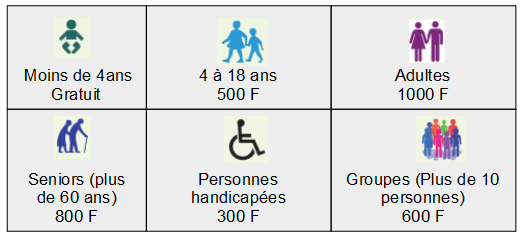
\includegraphics[scale=0.5]{images/tarif_parc1.png}
\end{center}


\end{multicols}

\end{enumerate}
\end{exo}

\vspace{0.5cm}

\begin{exo}
Un conducteur de camion conduit son véhicule pendant 6h par jour et met 3 jours parcourir 1000km. Donne une valeur approchée au dixième près de la vitesse horaire moyenne du camion.
\end{exo}

\vspace{0.5cm}
\begin{exo}
On vide un fût de 75l dans des bouteilles de 15dl. Combien de bouteille a-t-on utilisées?
\end{exo}

\vspace{0.5cm}

\begin{exo}
Recopie et complète par 10 ; 100 ; 1 000...
\begin{enumerate}
\begin{multicols}{2}
\item $8,79 \times \ldots = 87,9$
\item $4,35 \times \ldots = 43 500$
\item $0,837 \times \ldots = 8,37$
\item $0,367 \times \ldots = 3,67$
\item $0,028 \times \ldots = 0,28$
\item $0,17 \div \ldots= 0,017$
\item $23 \div \ldots = 0,23$
\item $480 \div \ldots = 4,8$
\item $900 \div \ldots = 0,09$
\item $18 000 \div \ldots = 18$
\end{multicols}
\end{enumerate}
\end{exo}

\begin{exo}
\setlength{\columnseprule}{1pt}
\begin{multicols}{2}
Observe cette figure composée de deux segments [AB] et [CD] sécants et indique pour chaque affirmation si elle est vraie ou fausse.
\begin{enumerate}
\item Les points C, D et M sont alignés.
\item M est le point d'intersection des segments [AB] et [CD].
\item M est le milieu du segment [AC].
\item M est un point du segment [CD].
\item A appartient au segment [MB].
\item M est le milieu du segment [CD].
\end{enumerate}
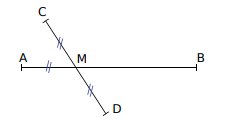
\includegraphics[scale=0.9]{images/td_29_02_20_img2.png}
\end{multicols}
\end{exo}
\end{td}
\end{document}
